\documentclass[11pt,a4paper,final]{article}
\usepackage[utf8]{inputenc}
\usepackage[portuguese]{babel}
\usepackage[T1]{fontenc}
\usepackage{amsmath}
\usepackage{amsfonts}
\usepackage{amssymb}
\usepackage{graphicx}
\graphicspath{ {figs/} }
\usepackage{caption}
\usepackage{subcaption}
\usepackage{pstricks,pst-osci,pst-circ}
\usepackage[left=2cm,right=2cm,top=1cm,bottom=2cm]{geometry}
\author{Tiago \'{A}. Oliveira}
\title{Proposta de Resolu\c{c}\~{a}o do Relat\'{o}rio Individual}
\begin{document}
\begin{center}
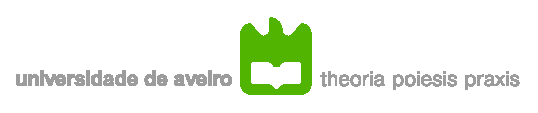
\includegraphics[scale=1]{logo_UA}
\linebreak\linebreak
\LARGE\textbf{Eletricidade \& Magnetismo}
\normalsize\linebreak
(2013-2014)
\linebreak\linebreak
\textbf{Proposta de Resolu\c{c}\~{a}o do Relat\'{o}rio Individual de Laborat\'{o}rio}
\linebreak
10 de dezembro de 2013
\linebreak\linebreak
\textcolor{red}{\underline{Vers\~{a}o A}} \& \textcolor{blue}{\underline{Vers\~{a}o B}}
\end{center}

\noindent\textbf{1) Eletroest\'{a}tica} \hfill [\textit{3 valores}]

Quando o aluno eletriza por fric\c{c}\~{a}o uma barra de \textcolor{red}{acr\'{i}lico} / \textcolor{blue}{PVC} esta fica carregada \textcolor{red}{positivamente} / \textcolor{blue}{negativamente} na zona em que foi friccionada. O pano usado fica por sua vez carregado com carga oposta.

Inicialmente o eletrosc\'{o}pio encontra-se descarregado. Ao aproximar a barra da cabe\c{c}a do eletrosc\'{o}pio, por indu\c{c}\~{a}o eletrost\'{a}tica, esta fica carregada \textcolor{red}{negativamente} / \textcolor{blue}{positivamente}. Como h\'{a} um fluxo de cargas \textcolor{red}{negativas} / \textcolor{blue}{positivas} para a cabe\c{c}a do eletrosc\'{o}pio, as palhetas (na outra extremidade) ficam com excesso de cargas \textcolor{red}{positivas} / \textcolor{blue}{negativas}.

\begin{figure}[h]
\centering
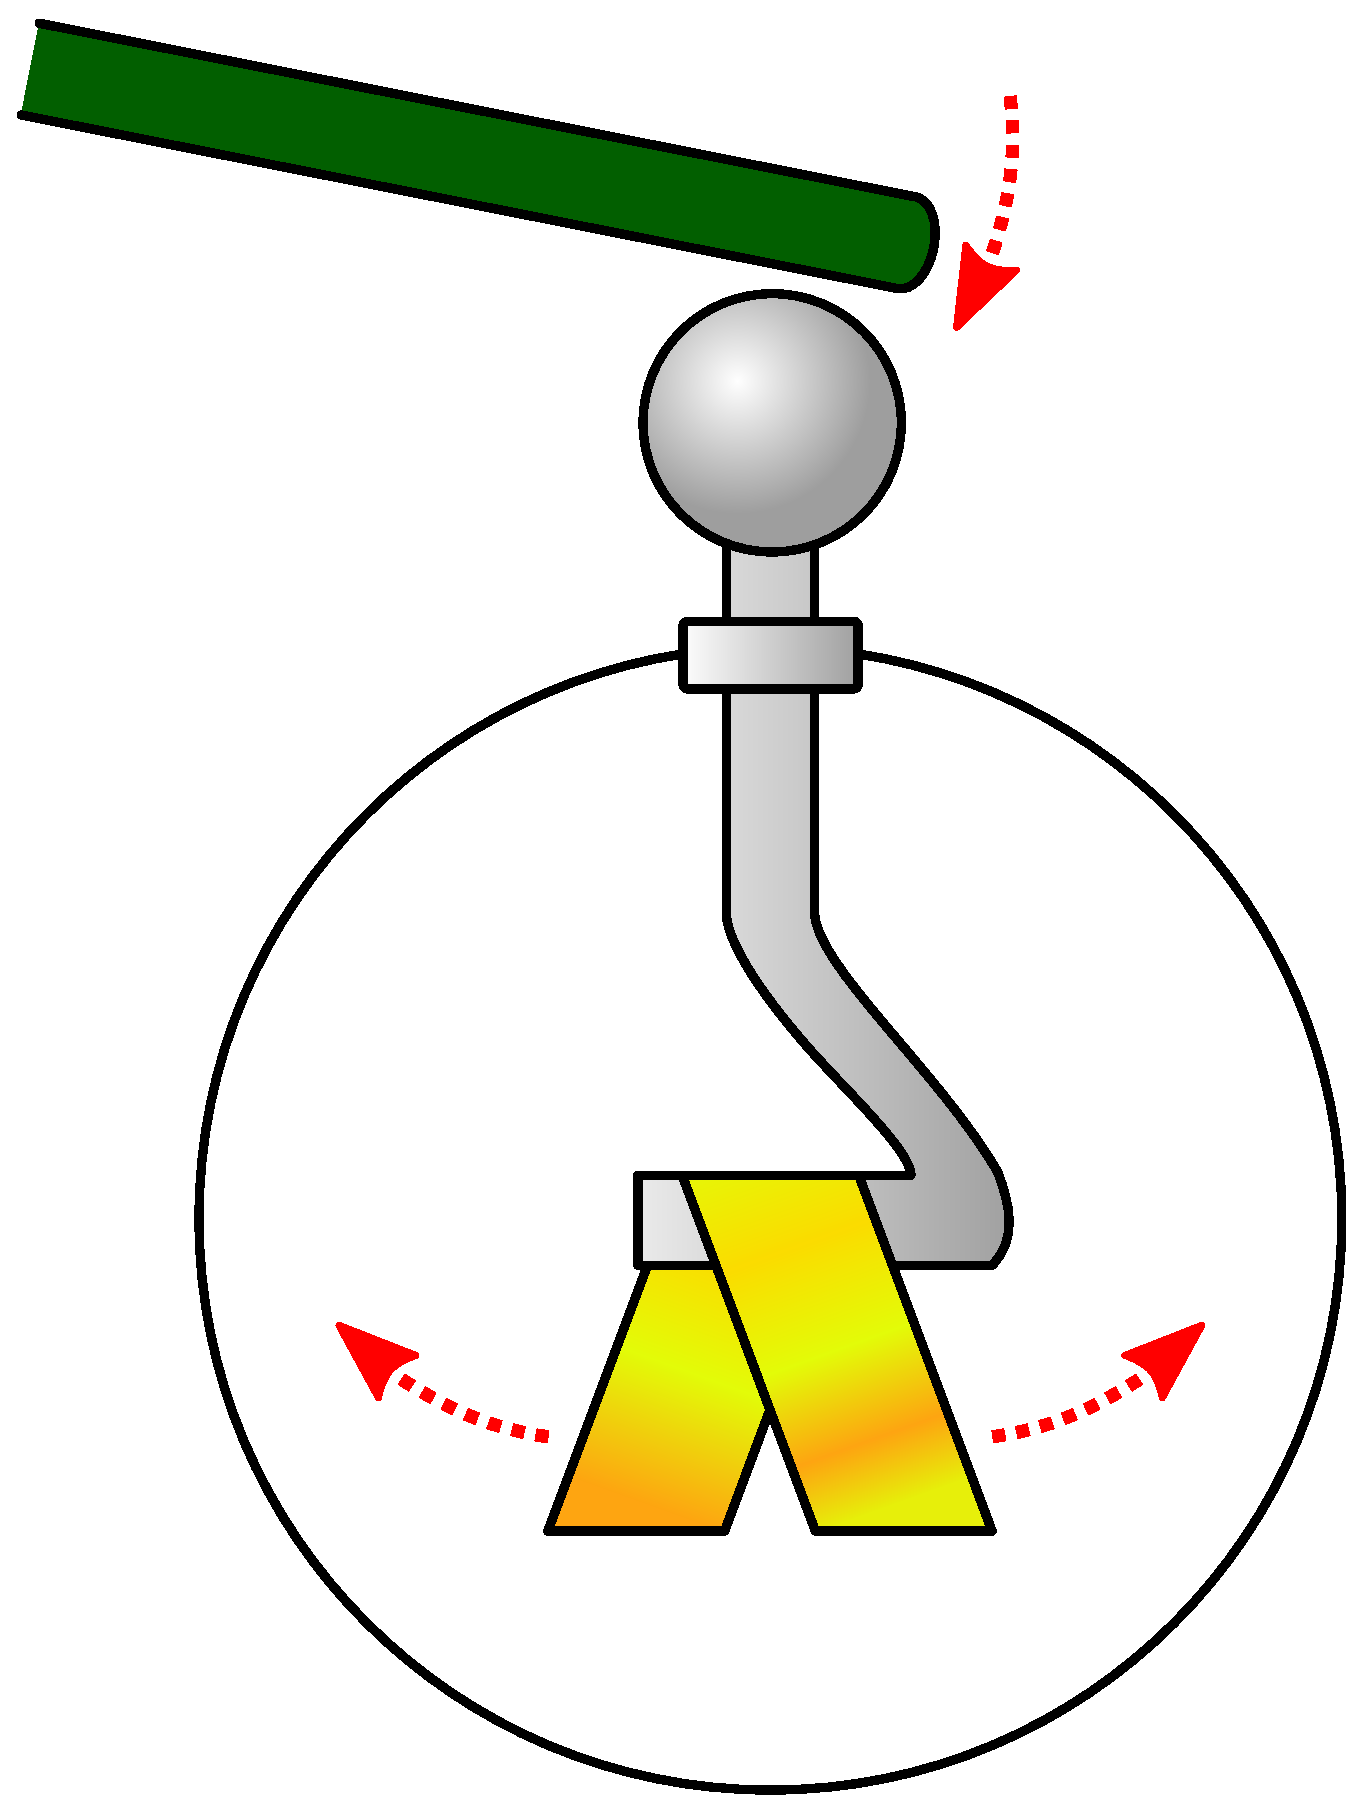
\includegraphics[scale=0.2]{electroscope.eps}
\caption{\label{fig:eletroscopio}Eletrosc\'{o}pio de palhetas.}
\end{figure}

Como as duas palhetas finas e de massa muito pequena ficam ambas carregadas com a mesma carga, devido \`{a} for\c{c}a eletrost\'{a}tica repulsiva entre as cargas de mesmo sinal, as palhetas afastam-se uma da outra (Fig.~\ref{fig:eletroscopio}). Este fen\'{o}meno ocorre, independentemente da carga induzida, logo \'{e} imposs\'{i}vel avaliar o sinal da carga induzida na cabe\c{c}a do eletrosc\'{o}pio.

Ao tocar com a barra de \textcolor{red}{acr\'{i}lico} / \textcolor{blue}{PVC} na cabe\c{c}a do eletrosc\'{o}pio, como s\~{a}o de material mau condutor, as cargas presentes na cabe\c{c}a n\~{a}o ir\~{a}o fluir totalmente para a barra. Ao afastar-se a barra da cabe\c{c}a, o eletrosc\'{o}pio tende para o equil\'{i}brio eletrost\'{a}tico. Se parte da carga tiver sido descarregada pela barra aquando do contacto, uma carga residual permanece nas palhetas e elas permanecem afastadas.

~\linebreak
\noindent\textbf{2) Circuitos de corrente cont\'{i}nua} \hfill [\textit{2 valores}]

Determinar o circuito equivalente de Th\'{e}venin consiste em simplificar o circuito esquematizado na Fig.~1 do enunciado num circuito constitu\'{i}do por uma fonte de tens\~{a}o ligada em s\'{e}rie com uma resistência, como mostra a Fig.~\ref{fig:circthev}.

\begin{figure}[h]
\begin{center}
\begin{pspicture}[showgrid=false](5,4)
\pnode(1,0){A}
\pnode(1,3){B}
\pnode(4,0){b}
\pnode(4,3){a}
\vdc[labeloffset=-1.0](B)(A){$V_{Th}$}
\resistor[dipolestyle=zigzag,arrows=-o](B)(a){$R_{Th}$}
\wire[arrows=-o](A)(b)
\uput[r](a){$A$}
\uput[r](b){$B$}
\end{pspicture}
\end{center}
\caption{\label{fig:circthev}Circuito equivalente de Th\'{e}venin}
\end{figure}

Para determinar $V_{Th}$ precisamos de calcular a queda de tens\~{a}o, em circuito aberto, entre os nodos $A$ e $B$ do circuito original e para determinar $R_{Th}$ "curto-circuita-se"~a fonte de tens\~{a}o do circuito original e determina-se a resist\^{e}ncia equivalente entre os mesmos nodos.

Em ambas as vers\~{o}es, no circuito original encontram-se duas resist\^{e}ncias associadas em paralelo de $2.2~\text{k}\Omega$ e de $220~\Omega$. A resist\^{e}ncia equivalente \`{a} associa\c{c}\~{a}o de ambas ser\'{a}:

\begin{equation*}
R_{eq}=\frac{1}{\frac{1}{220}+\frac{1}{2.2\times10^3}}
=\frac{1}{\frac{2.2\times10^3+220}{220\times2.2\times10^3}}
=\frac{220\times2.2\times10^3}{2.2\times10^3+220}
=200~\Omega
\end{equation*}

Logo, por uma quest\~{a}o de simplifica\c{c}\~{a}o, em ambas as vers\~{o}es esta associa\c{c}\~{a}o em paralelo pode ser substitu\'{i}da por uma resist\^{e}ncia de $200~\Omega$.

~\linebreak
\noindent$R_{Th}$ :

Se substituirmos a fonte de tens\~{a}o por um curto-circuito e tendo em conta a simplifica\c{c}\~{a}o anterior, o circuito original ter\'{a} a disposi\c{c}\~{a}o de resist\^{e}ncias da Fig.~\ref{fig:rth}.

\begin{figure}[h]
        \centering
        \begin{subfigure}[b]{0.5\textwidth}
                \begin{pspicture}[showgrid=false](8,4)
				\pnode(1,0){A}
				\pnode(4,0){B}
				\pnode(7,0){C}
				\pnode(1,3){D}
				\pnode(4,3){E}
				\pnode(7,3){a}
				\pnode(7,0){b}
				%\vdc[labeloffset=-1.4](D)(A){$15.0~\text{V}$}
				\wire[arrows=*-*,linecolor=red](D)(A)
				\resistor[dipolestyle=zigzag,linecolor=red](D)(E){$200$}
				\resistor[dipolestyle=zigzag](E)(B){$1\text{k}5$}
				\resistor[dipolestyle=zigzag,arrows=-o](E)(a){$100$}
				\wire[arrows=*-o](B)(b)
				\wire(A)(B)
				\uput[r](a){$A$}
				\uput[r](b){$B$}
				\end{pspicture}
                \caption{\textcolor{red}{\underline{Vers\~{a}o A}}}
        \end{subfigure}%
        ~ %add desired spacing between images, e. g. ~, \quad, \qquad etc.
          %(or a blank line to force the subfigure onto a new line)
        \begin{subfigure}[b]{0.5\textwidth}
				\begin{pspicture}[showgrid=false](8,4)
				\pnode(1,0){A}
				\pnode(4,0){B}
				\pnode(7,0){C}
				\pnode(1,3){D}
				\pnode(4,3){E}
				\pnode(7,3){a}
				\pnode(7,0){b}
				%\vdc[labeloffset=-1.4](D)(A){$15.0~\text{V}$}
				\wire[arrows=*-*,linecolor=blue](D)(A)
				\resistor[dipolestyle=zigzag](D)(E){$1\text{k}5$}
				\resistor[dipolestyle=zigzag,linecolor=blue](E)(B){$200$}
				\resistor[dipolestyle=zigzag,arrows=-o](E)(a){$470$}
				\wire[arrows=*-o](B)(b)
				\wire(B)(A)
				\uput[r](a){$A$}
				\uput[r](b){$B$}
				\end{pspicture}
                \caption{\textcolor{blue}{\underline{Vers\~{a}o B}}}
        \end{subfigure}
        \caption{Associa\c{c}\~{a}o de resist\^{e}ncias para determinar $R_{Th}$}\label{fig:rth}
\end{figure}

Nestas condi\c{c}\~{o}es, a resist\^{e}ncia equivalente de $200~\Omega$ encontra-se associada em paralelo com a resist\^{e}ncia de $1.5~\text{k}\Omega$, que por sua vez encontram-se ambas associadas em série com a resistência de $\color{red}100~\Omega$ / $\color{blue}470~\Omega$. Vamos ent\~{a}o definir $R_{eq}'=200\parallel1\text{k}5$,

\begin{equation*}
R_{eq}'=\frac{1}{\frac{1}{200}+\frac{1}{1.5\times10^3}}
=\frac{1}{\frac{1.5\times10^3+200}{200\times1.5\times10^3}}
=\frac{200\times1.5\times10^3}{1.5\times10^3+200}
=\frac{3000}{17}~\Omega
\end{equation*}

\noindent\textcolor{red}{\underline{Vers\~{a}o A} : }

\begin{equation*}
\color{red}R_{Th}=\frac{3000}{17}+100=\frac{4700}{17}\Rightarrow
\boxed{R_{Th}\approx276~\Omega}
\end{equation*}

\noindent\textcolor{blue}{\underline{Vers\~{a}o B} : }
\begin{equation*}
\color{blue}R_{Th}=\frac{3000}{17}+470=\frac{10990}{17}\Rightarrow
\boxed{R_{Th}\approx646~\Omega}
\end{equation*}

~\linebreak
\noindent$V_{Th}$ :

Como a tens\~{a}o de Th\'{e}venin ($V_{Th}$) \'{e} a tens\~{a}o em \underline{circuito aberto} entre os nodos $A$ e $B$, logo n\~{a}o existe corrente a fluir na resist\^{e}ncia de $\color{red}100~\Omega$ / $\color{blue}470~\Omega$. Assim n\~{a}o ocorre uma quebra de tens\~{a}o nesta resist\^{e}ncia.

Para a determina\c{c}\~{a}o de $V_{Th}$, necessitamos apenas de analisar o circuito da Fig.~\ref{fig:vth}, que nas aulas pr\'{a}ticas vulgarmente denomin\'{a}vamos por divisor resistivo.

\begin{figure}[h]
        \centering
        \begin{subfigure}[b]{0.5\textwidth}
        \centering
                \begin{pspicture}[showgrid=false](7,5)
				\pnode(1,0){A}
				\pnode(4,0){B}
				\pnode(1,3){D}
				\pnode(4,3){E}
				\pnode(6,3){a}
				\pnode(6,0){b}
				\vdc[labeloffset=-1.2,tension,tensionstyle=pm](D)(A){$15.0~\text{V}$}
				\resistor[dipolestyle=zigzag,labeloffset=-0.6,
				          linecolor=red,
				          intensitylabel=$\color{purple}i$,
				          intensitycolor=purple,
				          intensitywidth=3\pslinewidth,
				          tensionlabel=$\color{orange}V'$,
				          tensionstyle=pm,
				          tensioncolor=orange](D)(E){$200$}
				\resistor[dipolestyle=zigzag,labeloffset=-0.7,
				          intensitylabel=$\color{purple}i$,
				          intensitycolor=purple,
				          tension,
				          tensionstyle=pm,
				          intensitywidth=3\pslinewidth](E)(B){$1\text{k}5$}
				\wire[arrows=*-o,
				          linecolor=red,
				          intensitylabel=$\color{purple}i{=}0$,
				          intensitycolor=purple,
				          intensitywidth=3\pslinewidth](E)(a)
				\wire[arrows=*-o](B)(b)
				\wire(A)(B)
				\uput[r](a){$A$}
				\uput[r](b){$B$}
				\tension[tensioncolor=orange](a)(b){$\color{orange}V_{Th}$}
				\end{pspicture}
                \caption{\textcolor{red}{\underline{Vers\~{a}o A}}}
        \end{subfigure}%
        ~ %add desired spacing between images, e. g. ~, \quad, \qquad etc.
          %(or a blank line to force the subfigure onto a new line)
        \centering
        \begin{subfigure}[b]{0.5\textwidth}
                \begin{pspicture}[showgrid=false](7,5)
				\pnode(1,0){A}
				\pnode(4,0){B}
				\pnode(1,3){D}
				\pnode(4,3){E}
				\pnode(6,3){a}
				\pnode(6,0){b}
				\vdc[labeloffset=-1.2,tension,tensionstyle=pm](D)(A){$15.0~\text{V}$}
				\resistor[dipolestyle=zigzag,labeloffset=-0.6,
				          intensitylabel=$\color{purple}i$,
				          intensitycolor=purple,
				          intensitywidth=3\pslinewidth,
				          tensionlabel=$\color{orange}V'$,
				          tensionstyle=pm,
				          tensioncolor=orange](D)(E){$1\text{k}5$}
				\resistor[dipolestyle=zigzag,labeloffset=-0.7,
				          linecolor=blue,
				          intensitylabel=$\color{purple}i$,
				          intensitycolor=purple,
				          tension,
				          tensionstyle=pm,
				          intensitywidth=3\pslinewidth](E)(B){$200$}
				\wire[arrows=*-o,
				          linecolor=blue,
				          intensitylabel=$\color{purple}i{=}0$,
				          intensitycolor=purple,
				          intensitywidth=3\pslinewidth](E)(a)
				\wire[arrows=*-o](B)(b)
				\wire(A)(B)
				\uput[r](a){$A$}
				\uput[r](b){$B$}
				\tension[tensioncolor=orange](a)(b){$\color{orange}V_{Th}$}
				\end{pspicture}
                \caption{\textcolor{blue}{\underline{Vers\~{a}o B}}}
        \end{subfigure}
        \caption{An\'{a}lise do divisor resistivo para determinar $V_{Th}$}\label{fig:vth}
\end{figure}

Usando as leis de Kirchhoff para analisar o circuito da Fig.~\ref{fig:vth}, verificamos que a corrente $i$ que flui na resist\^{e}ncia de $200~\Omega$ \'{e} igual \'{a} corrente que flui na resist\^encia de $1.5~\text{k}\Omega$, logo obtemos a seguinte igualdade a partir da lei de Ohm,

\noindent\textcolor{red}{\underline{Vers\~{a}o A} : }

\begin{equation*}
\color{red}i=\frac{V'}{200}=\frac{V_{Th}}{1.5\times10^3}\Rightarrow
V'=\frac{200}{1.5\times10^3}V_{Th}
\end{equation*}

\noindent\textcolor{blue}{\underline{Vers\~{a}o B} : }

\begin{equation*}
\color{blue}i=\frac{V'}{1.5\times10^3}=\frac{V_{Th}}{200}\Rightarrow
V'=\frac{1.5\times10^3}{200}V_{Th}
\end{equation*}

A partir da lei das malhas, a totalidade das subidas/quedas de tens\~{a}o ao longo de uma malha t\^{e}m de se anular, logo

\begin{equation*}
15.0-V'-V_{Th}=0 \Leftrightarrow V'=15.0-V_{Th}
\end{equation*}

Igualando a express\~{a}o anterior com a obtida a partir da lei dos n\'{o}s,

\noindent\textcolor{red}{\underline{Vers\~{a}o A} : }

\begin{equation*}
\color{red}\frac{200}{1.5\times10^3}V_{Th}=15.0-V_{Th} \Leftrightarrow
\frac{200}{1.5\times10^3}V_{Th}+V_{Th}=15.0 \Leftrightarrow
\left[\frac{200}{1.5\times10^3}+1\right]V_{Th}=15.0 \Leftrightarrow
\end{equation*}

\begin{equation*}
\color{red}\frac{200+1.5\times10^3}{1.5\times10^3}V_{Th}=15.0 \Leftrightarrow
V_{Th}=15.0\frac{1.5\times10^3}{200+1.5\times10^3} \Leftrightarrow
V_{Th}=\frac{225}{17} \Rightarrow
\boxed{V_{Th}\approx13.2~\text{V}}
\end{equation*}

\noindent\textcolor{blue}{\underline{Vers\~{a}o B} : }

\begin{equation*}
\color{blue}\frac{1.5\times10^3}{200}V_{Th}=15.0-V_{Th} \Leftrightarrow
\frac{1.5\times10^3}{200}V_{Th}+V_{Th}=15.0 \Leftrightarrow
\left[\frac{1.5\times10^3}{200}+1\right]V_{Th}=15.0 \Leftrightarrow
\end{equation*}

\begin{equation*}
\color{blue}\frac{200+1.5\times10^3}{200}V_{Th}=15.0 \Leftrightarrow
V_{Th}=15.0\frac{200}{200+1.5\times10^3} \Leftrightarrow
V_{Th}=\frac{30}{17} \Rightarrow
\boxed{V_{Th}\approx1.76~\text{V}}
\end{equation*}

O circuito equivalente de Th\'{e}venin do original ser\'{a} ent\~{a}o o representado na Fig.~\ref{fig:thevenin}.

\begin{figure}[h]
        \centering
        \begin{subfigure}[b]{0.5\textwidth}
		\centering		
		\begin{pspicture}[showgrid=false](5,4)
		\pnode(1,0){A}
		\pnode(1,3){B}
		\pnode(4,0){b}
		\pnode(4,3){a}
		\vdc[labeloffset=-1.2,linecolor=red](B)(A){$\color{red}13.2~\text{V}$}
		\resistor[dipolestyle=zigzag,linecolor=red,arrows=-o](B)(a){$\color{red}276~\Omega$}
		\wire[arrows=-o](A)(b)
		\uput[r](a){$A$}
		\uput[r](b){$B$}
		\end{pspicture}
        \caption{\textcolor{red}{\underline{Vers\~{a}o A}}}
        \end{subfigure}%
        ~ %add desired spacing between images, e. g. ~, \quad, \qquad etc.
          %(or a blank line to force the subfigure onto a new line)
        \begin{subfigure}[b]{0.5\textwidth}
		\centering
		\begin{pspicture}[showgrid=false](5,4)
		\pnode(1,0){A}
		\pnode(1,3){B}
		\pnode(4,0){b}
		\pnode(4,3){a}
		\vdc[labeloffset=-1.2,linecolor=blue](B)(A){$\color{blue}1.76~\text{V}$}
		\resistor[dipolestyle=zigzag,linecolor=blue,arrows=-o](B)(a){$\color{blue}646~\Omega$}
		\wire[arrows=-o](A)(b)
		\uput[r](a){$A$}
		\uput[r](b){$B$}
		\end{pspicture}
        \caption{\textcolor{blue}{\underline{Vers\~{a}o B}}}
        \end{subfigure}
        \caption{Circuitos equivalentes aos circuitos originais.}\label{fig:thevenin}
\end{figure}

~\linebreak
\noindent\textbf{3) Bobinas de Helmholtz} %\hfill [\textit{7,5 valores}]

\textbf{a)} \hfill [\textit{3 valores}]

O efeito de Hall consiste na produ\c{c}\~{a}o de uma diferen\c{c}a de potencial (Tens\~{a}o de Hall) atrav\'{e}s de um condutor el\'{e}trico, geralmente um semicondutor, transversal \`{a} corrente el\'{e}trica no condutor e a um campo magn\'{e}tico perpendicular \`{a} corrente (ver Fig.\ref{fig:hall}).

Num semicondutor, esta corrente \'{e} devida aos portadores de carga maiorit\'{a}rios, tipicamente eletr\~{o}es (carga negativa) ou lacunas (carga positiva). Quando um campo magn\'{e}tico est\'{a} presente e n\~{a}o \' {e} paralelo \`{a} dire\c{c}\~{a}o de movimento dos portadores de carga, estes sofrem a a\c{c}\~{a}o de uma for\c{c}a (for\c{c}a de Lorentz). Na aus\^{e}ncia de tal campo magn\'{e}tico, os portadores de carga fluiriam aproximadamente em trajet\'{o}ria retil\'{i}nea. Contudo, quando um campo magn\'{e}tico com uma componente perpendicular \'{e} aplicado, a sua trajet\'{o}ria tende a curvar de modo que as cargas come\c{c}am a acumular numa das faces do material. Por consequ\^{e}ncia, cargas de sinal oposto acumular\~{a}o na face oposta. O resultado \'{e} uma distribui\c{c}\~{a}o assim\'{e}trica de densidade de carga ao longo do elemento do condutor, simultaneamente perpendicular \`{a} corrente de portadores de carga e do campo magn\'{e}tico aplicado. A separa\c{c}\~{a}o de cargas estabelece um campo el\'{e}trico que se op\~{o}e \`{a} evolu\c{c}\~{a}o da migra\c{c}\~{a}o de carga, logo em equil\'{i}brio uma diferen\c{c}a de potencial el\'{e}trico \'{e} estabelecida desde que se mantenha o fluxo de portadores de carga. Esta diferen\c{c}a de potencial \'{e} proporcional \`{a} componente perpendicular do campo magn\'{e}tico aplicado.

\begin{figure}[h]
\centering
\begin{pspicture}[showgrid=false](-6,-6)(8,4)

% Sample
\psline[linewidth=2pt]{c-c}(-4.5,2)(3.5,2)
\psline[linewidth=2pt]{c-c}(3.5,2)(3.5,-3)
\psline[linewidth=2pt]{c-c}(-4.5,-3)(-4.5,2)
\psline[linewidth=2pt]{c-c}(-4.5,-3)(3.5,-3)
\psline[linewidth=2pt]{c-c}(-4.5,2)(-3.5,3)
\psline[linewidth=2pt,linestyle=dashed]{c-c}(-4.5,-3)(-3.5,-2)
\psline[linewidth=2pt,linestyle=dashed]{c-c}(-3.5,-2)(-3.5,3)
\psline[linewidth=2pt,linestyle=dashed]{c-c}(-3.5,-2)(4.5,-2)
\psline[linewidth=2pt]{c-c}(3.5,-3)(4.5,-2)
\psline[linewidth=2pt]{c-c}(3.5,2)(4.5,3)
\psline[linewidth=2pt]{c-c}(4.5,-2)(4.5,3)
\psline[linewidth=2pt]{c-c}(-3.5,3)(4.5,3)

% Vectors
\psline[linewidth=2pt,linecolor=blue]{->}(-2.5,0)(-1,0)
\psline{(->}(-2.4,0.1)(-1,1.5)
\psline{(->}(2.6,0.1)(4,1.5)
\cput[linestyle=none](-1,-.5){$\color{blue}{\overrightarrow{v_d}}$}
\psline[linewidth=2pt,linecolor=blue]{->}(-2.5,0)(-2.5,1.5)
\rput(-4.5,1.5){\psframebox*[framearc=.3,opacity=0.85]{$\color{blue}{\overrightarrow{F_M}=+q\overrightarrow{v_d}\times\overrightarrow{B}}$}}
\psline[linewidth=2pt,linecolor=blue]{->}(-2.5,0)(-2.5,-1.5)
\rput(-4,-1.5){\psframebox*[framearc=.3,opacity=0.85]{$\color{blue}{\overrightarrow{F_E}=+q\overrightarrow{E}}$}}
\psline[linewidth=2pt,linecolor=red]{->}(2.5,0)(1,0)
\cput[linestyle=none](1,-.5){$\color{red}{\overrightarrow{v_d}}$}
\psline[linewidth=2pt,linecolor=red]{->}(2.5,0)(2.5,1.5)
\rput(4.5,1.5){\psframebox*[framearc=.3,opacity=0.85]{$\color{red}{\overrightarrow{F_M}=-q\overrightarrow{v_d}\times\overrightarrow{B}}$}}
\psline[linewidth=2pt,linecolor=red]{->}(2.5,0)(2.5,-1.5)
\rput(4,-1.5){\psframebox*[framearc=.3,opacity=0.85]{$\color{red}{\overrightarrow{F_E}=-q\overrightarrow{E}}$}}

\psbezier[linestyle=dashed]{->}(-2.5,0)(-2.0,0)(-0.5,0)(-0.5,1.5)
\psbezier[linestyle=dashed]{->}(2.5,0)(2.0,0)(0.5,0)(0.5,1.5)
\rput(0,.6){\psframebox*[framearc=.3,opacity=0.85]{\begin{tabular}{c}trajet\'{o}ria \\ inicial\end{tabular}}}

\cput[fillstyle=solid,fillcolor=white,opacity=0.85,linecolor=blue](-2.5,0){$\color{blue}{+}$}
\cput[fillstyle=solid,fillcolor=white,opacity=0.85,linecolor=red](2.5,0){$\color{red}{-}$}
\multirput(-3.5,2.5)(.5,0){7}{$\color{blue}{+}$}
\multirput(-3.5,-2.5)(.5,0){7}{$\color{blue}{-}$}
\multirput(3.5,2.5)(-.5,0){7}{$\color{red}{-}$}
\multirput(3.5,-2.5)(-.5,0){7}{$\color{red}{+}$}
\psline[linecolor=blue]{->}(-1.5,-.5)(-1.5,-2)
\rput(-1,-1.5){$\color{blue}{\overrightarrow{E}}$}
\psline[linecolor=red]{->}(1.5,-2)(1.5,-.5)
\rput(2,-1.5){$\color{red}{\overrightarrow{E}}$}
\psline[border=1pt]{-)}(-4,-1.5)(-2.6,-0.1)
\psline[border=1pt]{-)}(1,-1.5)(2.4,-0.1)
\rput(-2,1){$\overrightarrow{B}$}

% Circuit
\pnode(-5,-4.5){A}
\pnode(5,-4.5){B}
\pnode(-5,0){C}
\pnode(-4.5,0){cc}
\pnode(-4,0){c}
\pnode(5,0){D}
\pnode(4,0){d}
\pnode(0,2.5){f}
\pnode(0,3.5){F}
\pnode(6.5,3.5){G}
\pnode(0,-2.5){h}
\pnode(0,-3){hh}
\pnode(0,-3.5){H}
\pnode(6.5,-3.5){I}
\Ucc[labelInside=1,labeloffset=1](B)(A){$I_H$}
\wire[intensity,intensitywidth=3\pslinewidth](A)(C)
\wire[intensity,intensitywidth=3\pslinewidth](D)(B)
\wire[arrows=-*,linestyle=dashed](cc)(c)
\wire[arrows=-*,linestyle=dashed](hh)(h)
\wire(H)(hh)
\wire(C)(cc)
\wire[arrows=*-](d)(D)
\wire[arrows=*-](f)(F)
\wire[arrows=-o](F)(G)
\wire(H)(4.5,-3.5)
\wire[intersect,intersectA=D,intersectB=B](4.5,-3.5)(5.5,-3.5)
\wire[arrows=-o](5.5,-3.5)(I)
\tension(G)(I){$V_H$}
\end{pspicture}
\caption{\label{fig:hall}Efeito de Hall num semicondutor.}
\end{figure}

\textbf{b)} \hfill [\textit{2,5 valores}]

A partir dos valores experimentais fornecidos e usando a express\~{a}o do campo magn\'{e}tico no interior do solenoide $B_S$, a representa\c{c}\~{a}o gr\'{a}fica da tens\~{a}o de Hall $V_H$ em fun\c{c}\~{a}o de $B_S$ encontra-se na Fig.~\ref{fig:calibracao}. Notem que os pontos experimentais t\^{e}m uma barra de erro ao longo de $x$. Isto deve-se ao facto de o campo magn\'{e}tico n\~{a}o ser uma medi\c{c}\~{a}o direta mas sim um calculo a partir da corrente efetivamente medida. Este c\'{a}lculo est\'{a} sujeito a uma incerteza que reflete assim as barras de erro representadas. Este aspeto \'{e} puramente opcional, n\~{a}o sendo exigida aquando da realiza\c{c}\~{a}o do relat\'{o}rio individual.

\begin{figure}[h]
\centering
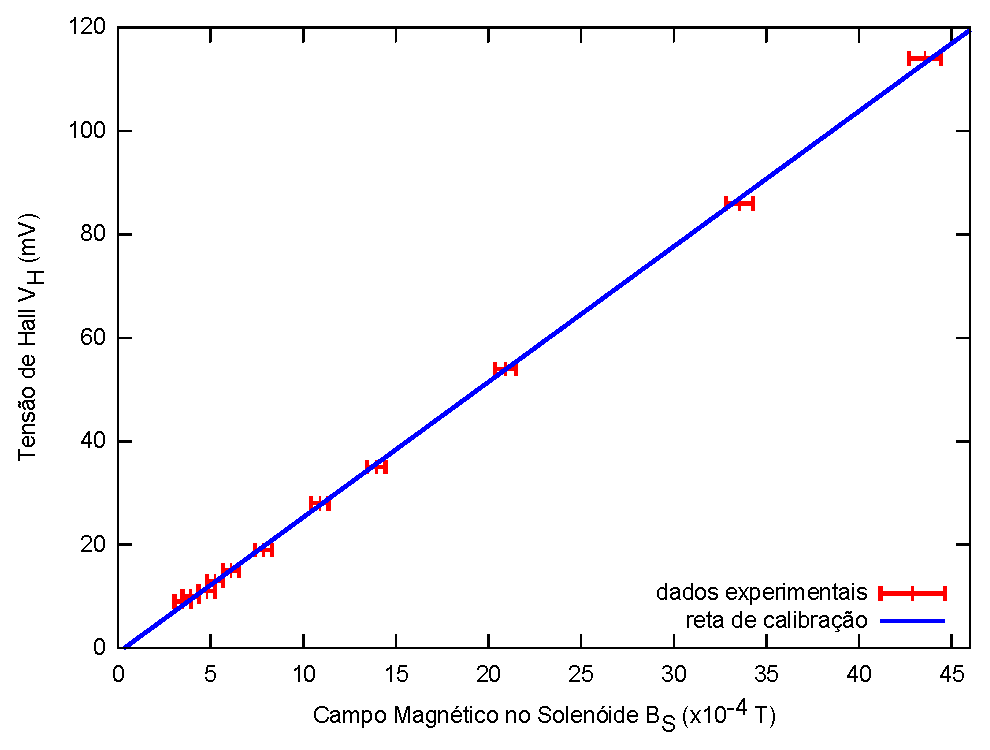
\includegraphics[scale=1]{calibracao.eps}
\caption{\label{fig:calibracao}Tens\~{a}o de Hall em fun\c{c}\~{a}o do campo magn\'{e}tico no interior do solenoide.}
\end{figure}

Para a calibra\c{c}\~{a}o dever\~{a}o recordar o final da resposta \`{a} al\'{i}nea anterior. O objetivo da calibra\c{c}\~{a}o da sonda \'{e} determinar a constante de proporcionalidade entre o campo magn\'{e}tico $B_S$ e a tens\~{a}o de Hall $V_H$.
\begin{equation*}
B_S=C_cV_H
\end{equation*}
Como podem verificar n\~{a}o podemos obter a constante de calibração $C_c$ aplicando diretamente o m\'{e}todo dos m\'{i}nimos desvios quadr\'{a}ticos (MMDQ) dos dados apresentados na Fig.~\ref{fig:calibracao}.

\underline{Esta era uma das "rasteiras"~presentes do enunciado!}

Mas se fizerem corresponder $V_H$ \`{a} vari\'{a}vel $x$, $B_S$ \`{a} vari\'{a}vel $y$ e aproximarem os valores experimentais a uma reta do tipo $y=mx+b$ pelo MMDQ, rapidamente obtemos a igualdade $C_c \pm \Delta C_c = m \pm \Delta m$.

Em resultado do MMDQ, obteriam os seguintes par\^{a}metros:
\begin{equation*}
m \pm \Delta m = \boxed{C_c \pm \Delta C_c = 38.2 \pm 0.2~(\text{mT/V})}
\end{equation*}
\begin{equation*}
b \pm \Delta b = 34.5 \pm 11.2~(\mu\text{V})
\end{equation*}
\begin{equation*}
r^2 = 0.99967692
\end{equation*}

\textbf{c)} \hfill [\textit{2 valores}]

Inicialmente precisamos de obter o campo magn\'{e}tico produzido pela bobina. Para isso recorremos \`{a} constante de calibra\c{c}\~{a}o obtida na al\'{i}nea anterior,
\begin{equation*}
B_\text{bobina}=C_cV_H \Rightarrow B_\text{bobina}=38.2\times10^{-3}\times50\times10^{-3}=1.91~\text{mT}
\end{equation*}
\begin{equation*}
\Delta B_\text{bobina}=\sqrt{\left[\frac{\partial B_\text{bobina}}{\partial C_c}\Delta C_c\right]^2+\left[\frac{\partial B_\text{bobina}}{\partial V_H}\Delta V_H\right]^2} = \sqrt{\left[V_H \Delta C_c\right]^2+\left[C_c\Delta V_H\right]^2} \Rightarrow
\end{equation*}
\begin{equation*}
\Delta B_\text{bobina}=0.04~\text{mT}
\end{equation*}
\begin{equation*}
\boxed{B_\text{bobina} \pm \Delta B_\text{bobina} =1.91 \pm 0.04~(\text{mT})}
\end{equation*}

Para determinar o campo magn\'{e}tico produzido por uma espira usa-se a express\~{a}o fornecida. O m\'{a}ximo do campo ocorre no plano da espira ($x=0$) logo,
\begin{equation*}
B_\text{espira}=\frac{\mu_0}{2}\frac{IR^2}{\left(R^2+0\right)^{3/2}} 
=\frac{\mu_0}{2}\frac{IR^2}{R^3}
=\frac{\mu_0}{2}\frac{I}{R}
\Rightarrow
B_\text{espira}=\frac{4\pi\times10^{-7}\times 0.50}{2\times3.5\times10^{-2}}
=8.98~\mu\text{T}
\end{equation*}
\begin{equation*}
\Delta B_\text{espira}=\sqrt{\left[\frac{\partial B_\text{espira}}{\partial I}\Delta I\right]^2+\left[\frac{\partial B_\text{espira}}{\partial R}\Delta R\right]^2} = \mu_0\sqrt{\left[\frac{\Delta I}{2R}\right]^2+\left[-\frac{ I \Delta R}{2R^2}\right]^2} \Rightarrow
\end{equation*}
\begin{equation*}
\Delta B_\text{espira}=4\pi\times10^{-7}\sqrt{\left[\frac{0.01}{2 \times 3.5 \times 10^{-2}}\right]^2+\left[-\frac{0.50 \times 0.1 \times 10^{-2}}{2 \left(3.5 \times 10^{-2}\right)^2}\right]^2}
=0.31~\mu\text{T}
\end{equation*}
\begin{equation*}
\boxed{B_\text{espira} \pm \Delta B_\text{espira} =8.98 \pm 0.31~(\mu\text{T})}
\end{equation*}

Por uma quest\~{a}o se simplifica\c{c}\~{a}o vamos supor que todas as espiras da bobina est\~{a}o no mesmo plano. Como o campo magn\'{e}tico obedece ao princ\'{i}pio da sobreposição, penso que ser\'{a} claro que facilmente obtemos a igualdade,
\begin{equation*}
B_\text{bobina}=nB_\text{espira} \Leftrightarrow
n=\frac{B_\text{bobina}}{B_\text{espira}}~\text{,}
\end{equation*}
\noindent em que $n$ \'{e} o n\'{u}mero de espiras.

\begin{equation*}
n=\frac{B_\text{bobina}}{B_\text{espira}} \Rightarrow
n=\frac{1.91 \times 10^{-3}}{8.98 \times 10^{-6}}=213~\text{espiras}
\end{equation*}
\begin{equation*}
\Delta n=\sqrt{\left[\frac{\partial n}{\partial B_\text{bobina}}\Delta B_\text{bobina}\right]^2+\left[\frac{\partial n}{\partial B_\text{espira}}\Delta B_\text{espira}\right]^2}
=\sqrt{\left[\frac{\Delta B_\text{bobina}}{B_\text{espira}}\right]^2+\left[-\frac{B_\text{bobina} \Delta B_\text{espira}}{\left(B_\text{espira}\right)^2}\right]^2}\Rightarrow
\end{equation*}
\begin{equation*}
\Delta n=\sqrt{\left[\frac{0.04 \times 10^{-3}}{8.98 \times 10^{-6}}\right]^2+\left[-\frac{1.91\times 10^{-3} \times 0.31 \times 10^{-6}}{\left(8.98 \times 10^{-6}\right)^2}\right]^2}
=9~\text{espiras}
\end{equation*}
\begin{equation*}
\boxed{n=213\pm9~(\text{espiras})}
\end{equation*}

~\linebreak
\noindent\textbf{4) Indu\c{c}\~{a}o} %\hfill [\textit{7,5 valores}]

\textbf{a)} \hfill [\textit{2,5 valores}]

Primeiro analisamos o Canal A (Fig. 2 do enunciado) onde se observa o sinal do \emph{prim\'{a}rio}. Precisamos de estimar $\frac{\mathrm d i}{\mathrm d t}$, mas como o oscilosc\'{o}pio n\~{a}o mede varia\c{c}\~{o}es de corrente, medimos a varia\c{c}\~{a}o de tens\~{a}o numa resist\^{e}ncia conhecida de $100~\Omega$.

\begin{equation*}
\Delta t \approx 4.0~\text{div}\times 0.15~\text{ms/div} \approx 0.60~\text{ms}
\end{equation*}
\begin{equation*}
\Delta V \approx 8.0~\text{div}\times 1.0~\text{V/div} \approx 8.0~\text{V}
\end{equation*}
Aplicando a lei de Ohm,
\begin{equation*}
\Delta V =R\Delta I\Leftrightarrow \Delta I = \frac{\Delta V}{R}\approx 80~\text{mA}
\end{equation*}
\begin{equation*}
\frac{\mathrm d i}{\mathrm d t}\approx\frac{\Delta I}{\Delta t}\Rightarrow\boxed{\frac{\mathrm d i}{\mathrm d t}\approx133~\text{A/s}}
\end{equation*}

\noindent f.e.m.:

Para determinar experimentalmente a f.e.m. induzida no \emph{secund\'{a}rio} basta determinar a amplitude do sinal medido pelo Canal~B do oscilosc\'{o}pio (Fig.~2 do enunciado), contudo o enunciado tem mais uma "rasteira". Como podiam verificar pelo par\^{a}metro "OffsetB" o zero n\~{a}o estava bem definido.
\begin{equation*}
2\varepsilon=3.0~\text{div} \times 0.2~\text{V/div}
\Rightarrow
\boxed{\varepsilon=0.3~\text{V}}
\end{equation*}

\noindent $M$:

\begin{equation*}
\varepsilon=M\frac{\mathrm d i}{\mathrm d t} \Rightarrow M=\frac{\varepsilon}{\frac{\mathrm d i}{\mathrm d t}}
\end{equation*}
\begin{equation*}
M_\text{experimental}=\frac{0.3}{133}\Rightarrow\boxed{M_\text{experimental}=2.26~\text{mH}}
\end{equation*}

A partir da Eq.~3 do enunciado,
\begin{equation*}
\frac{\varepsilon}{\frac{\mathrm d i}{\mathrm d t}}=M_\text{te\'{o}rico}=\pi\mu_0\frac{N}{l}r^2N_b \Rightarrow M_\text{te\'{o}rico}=\pi\times 4\pi \times 10^{-7} \times 3000 \times \left(1.38 \times 10^{-2}\right)^2\times 1200 \Rightarrow
\end{equation*}
\begin{equation*}
\boxed{M_\text{te\'{o}rico}=2.71~\text{mH}}
\end{equation*}

Alguns autores comparam valores experimentais com valores previstos para uma grandeza atrav\'{e}s de uma exactid\~{a}o definida da seguinte forma:

\begin{equation*}
\left|\frac{M_\text{experimental}-M_\text{te\'{o}rico}}{M_\text{te\'{o}rico}}\right|=\left|\frac{2.26-2.71}{2.71}\right|\approx 17\%
\end{equation*}

\textbf{b)} \hfill [\textit{2,5 valores}]

Para esbo\c{c}ar o sinal induzido no \emph{secund\'{a}rio} precisamos de saber a forma do sinal, a sua amplitude ($A$) e o seu per\'{i}odo ($T$).

Pela Eq.~3 no enunciado sabemos que a f.e.m. induzida no \emph{secund\'{a}rio} \'{e} proporcional \`{a} derivada em ordem ao tempo do sinal do \emph{prim\'{a}rio}. O sinal do tipo "dente-de-serra"~pode ser aproximado a uma sucess\~{a}o de segmentos de recta repetidos infinitamente, todos com o mesmo declive. Ora, nestes segmentos a derivada \'{e} simplesmente uma constante, como mostra a Fig.~\ref{fig:draft}. Contudo nos extremos, o sinal n\~{a}o \'{e} est\'{a}vel, logo a derivada apresenter\'{a} uma perturba\c{c}\~{o}es (Fig.~\ref{fig:draft} a tracejado). Aplicando um raciocinio semelhante \`{a} al\'{i}nea anterior, mas mantendo-nos afastados das extremidades.

\begin{equation*}
\Delta t \approx 4.0~\text{div}\times 0.05~\text{ms/div} \approx 0.20~\text{ms}
\end{equation*}
\begin{equation*}
\Delta V \approx 4.0~\text{div}\times 0.1~\text{V/div} \approx 0.4~\text{V}
\end{equation*}
Aplicando a lei de Ohm,
\begin{equation*}
\Delta V =R\Delta I\Leftrightarrow \Delta I = \frac{\Delta V}{R}\approx 4~\text{mA}
\end{equation*}
\begin{equation*}
\frac{\mathrm d i}{\mathrm d t}\approx\frac{\Delta I}{\Delta t}\Rightarrow\frac{\mathrm d i}{\mathrm d t}\approx20~\text{A/s}
\end{equation*}

Logo a f.e.m. (amplitude do sinal no \emph{secund\'{a}rio}),
\begin{equation*}
A=\varepsilon=M\frac{\mathrm d i}{\mathrm d t} \Rightarrow A=2.71\times10^{-3}\times 20 \Rightarrow \boxed{A\approx54~\text{mV}}
\end{equation*}

O per\'{i}odo no \emph{secund\'{a}rio} \'{e} o mesmo do sinal no \emph{prim\'{a}rio}, ou seja,
\begin{equation*}
T=5.2~\text{div}\times 0.05~\text{ms/div}\Rightarrow \boxed{T=0.26~\text{ms}}
\end{equation*}

\begin{figure}[h]
\centering
\begin{pspicture}[showgrid=false](-6,-4)(6,5)

% Sample
\psline{->}(-5,0)(5,0)
\psline{|-|}(-2.5,4)(3.5,4)
\psline[linewidth=2pt,linecolor=red]{c-c}(-5,2.4)(-3.5,2.4)
\psline[linewidth=2pt,linecolor=red,linestyle=dashed]{c-c}(-3.5,2.4)(-3,2)(-2.5,2.8)(-2,2)(-1.5,2.4)
\psline[linewidth=2pt,linecolor=red]{c-c}(-1.5,2.4)(2.5,2.4)
\psline[linewidth=2pt,linecolor=red,linestyle=dashed]{c-c}(2.5,2.4)(3,2)(3.5,2.8)(4,2)(4.5,2.4)
\psline[linewidth=2pt,linecolor=red]{c-c}(4.5,2.4)(5,2.4)

\psline[linecolor=red]{<->}(0,0)(0,2.4)
\psline[linecolor=blue]{<->}(0,0)(0,-2.4)
\psline[linewidth=2pt,linecolor=blue]{c-c}(-1.5,-2.4)(2.5,-2.4)
\psline[linewidth=2pt,linecolor=blue,linestyle=dashed]{c-c}(-3.5,-2.4)(-3,-2)(-2.5,-2.8)(-2,-2)(-1.5,-2.4)
\psline[linewidth=2pt,linecolor=blue]{c-c}(-5,-2.4)(-3.5,-2.4)
\psline[linewidth=2pt,linecolor=blue,linestyle=dashed]{c-c}(2.5,-2.4)(3,-2)(3.5,-2.8)(4,-2)(4.5,-2.4)
\psline[linewidth=2pt,linecolor=blue]{c-c}(4.5,-2.4)(5,-2.4)
\rput(0.5,4.5){$T$}
\rput(0.5,1.2){$\color{red}{A}$}
\rput(0.5,-1.2){$\color{blue}{-A}$}

\end{pspicture}
\caption{\label{fig:draft}Esbo\c{c}o do sinal indusido no \emph{secund\'{a}rio} na al\'{i}nea b).}
\end{figure}


\textbf{c)} \hfill [\textit{2,5 valores}]

Ao introduzir-se uma barra de \textcolor{red}{n\'{i}quel} / \textcolor{blue}{ferrite} estamos a alterar o meio do sistema f\'{i}sico. Podemos verificar que a permeabilidade magn\'{e}tica do meio \'{e} aproximadamente \textcolor{red}{99} / \textcolor{blue}{637} vezes superior \`{a} permeabilidade magn\'{e}tica inicial (do v\'{a}cuo).

\begin{equation*}
\color{red}\frac{\mu_{\text{n\'{i}quel}}}{\mu_0}=\frac{1.25\times10^{-4}~\text{H/m}}{4\pi\times10^{-7}~\text{H/m}}\approx99\qquad\color{blue}\frac{\mu_{\text{ferrite}}}{\mu_0}=\frac{8\times10^{-4}~\text{H/m}}{4\pi\times10^{-7}~\text{H/m}}\approx637
\end{equation*}

Facilmente se percebe, pela Eq.~3 do enunciado, que o coeficiente de indu\c{c}\~{a}o m\'{u}tua $M_{12}$ e, por conseguinte, a amplitude da for\c{c}a eletromotriz $\varepsilon$ ira sofrer um aumento da mesma ordem de grandeza.

\begin{equation*}
\color{red}\varepsilon_{\text{n\'{i}quel}}\approx99\varepsilon_\text{a)}\Rightarrow\boxed{\varepsilon_{\text{n\'{i}quel}}\approx30~\text{V}}
\qquad
\color{blue}\varepsilon_{\text{ferrite}}\approx637\varepsilon_\text{a)}\Rightarrow\boxed{\varepsilon_{\text{ferrite}}\approx191~\text{V}}
\end{equation*}

\end{document}